%\begin{figure}
%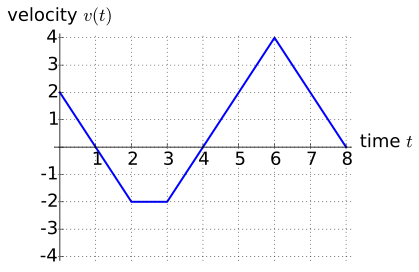
\includegraphics[width=\textwidth]{figs/4/activity_4-1-3a.pdf}
%\caption{The velocity function of a moving object.} \label{fig:activity_4-1-3a}
%\end{figure}

\begin{marginfigure}[6cm]
\margingraphics{figs/4/activity_4-1-3a.pdf}
\caption{The velocity function of a moving object.} \label{fig:activity_4-1-3a}
\end{marginfigure}

\begin{marginfigure}[0cm]
\margingraphics{figs/4/activity_4-1-3b.pdf}
\caption{The position function of a moving object.} \label{fig:activity_4-1-3b}
\end{marginfigure}

\begin{activity} \label{A:4.1.3}  Suppose that an object moving along a straight line path has its velocity $v$ (in meters per second) at time $t$ (in seconds) given by the piecewise linear function whose graph is pictured in Figure~\ref{fig:activity_4-1-3a}.  We view movement to the right as being in the positive direction (with positive velocity), while movement to the left is in the negative direction.

Suppose further that the object's initial position at time $t = 0$ is $s(0) = 1$.
\ba
\item Determine the total distance traveled and the total change in position on the time interval $0 \le t \le 2$.  What is the object's position at $t = 2$?

\item On what time intervals is the moving object's position function increasing?  Why?  On what intervals is the object's position decreasing?  Why?

\item What is the object's position at $t = 8$?  How many total meters has it traveled to get to this point (including distance in both directions)?  Is this different from the object's total change in position on $t = 0$ to $t = 8$?

\item Find the exact position of the object at $t = 1, 2, 3, \ldots, 8$ and use this data to sketch an accurate graph of $y = s(t)$ on the axes provided.  How can you use the provided information about $y = v(t)$ to determine the concavity of $s$ on each relevant interval?
\ea
\end{activity}

\begin{smallhint}
\ba
	\item Find the area of each triangular region formed between $y = v(t)$ and the $t$-axis.
	\item Recall that $v = s'$, and here we are given complete information about $v$.
	\item Be careful to address whether $v$ is positive or negative when calculating areas and adding the results.
	\item Consider finding the area bounded by $y = v(t)$ and the $t$-axis on each interval $[0,1]$, $[1,2]$, $\ldots$.
\ea
\end{smallhint}
\begin{bighint}
\ba
	\item Find the area of the triangular regions formed between $y = v(t)$ and the $t$-axis on $[0,1]$ and $[1,2]$.
	\item Recall that $v = s'$, and here we are given complete information about $v$.
	\item Be careful to address whether $v$ is positive or negative when calculating areas and adding the results.
	\item Consider finding the area bounded by $y = v(t)$ and the $t$-axis on each interval $[0,1]$, $[1,2]$, $\ldots$.
\ea
\end{bighint}
\begin{activitySolution}
\ba
	\item By finding the area of the triangular regions formed between $y = v(t)$ and the $t$-axis on $[0,1]$ and $[1,2]$ (each of which is $1$), it follows that the object's total distance traveled is $2$, while its change in position is $0$.  The latter is true since the net signed area bounded by $v$ on $[0,2]$ is $1 - 1 = 0$.
	\item The object's position is increasing wherever its velocity is positive, hence for $0 \le t < 1$ and $4 < 5 < 8>$.
	\item By calculating the area bounded by the curve, we find 1 unit of area on $[0,1]$, 4 units of area on $[1,4]$, and 8 units of area on $[4,8]$, thus the total distance traveled on $0 \le t \le 8$ is $D = 1 + 4 + 8$ meters.  As the change in position is given by the net signed area on this interval, we find that the change in position is
	$$s(8) - s(0) = 1 - 4 + 8 = 5 \ \mbox{m}.$$
	\item In the figure below, at left we list all of the areas bounded by $v$ on each one-unit subinterval.  Along with the given starting point that $s(0) = 1$, we use the resulting changes in position to plot points for the function $s$.  For instance, we know $s(1) - s(0) = 1$, hence $s(1) = 2$.  Similarly, $s(2) - s(1) = -1$, thus $s(2) = 1$.  Continuing across the interval, we generate the function $s$ that is pictured at right.  Note that the portion of $s$ from $t = 2$ to $t = 3$ is linear because $v$ is constant there, while the other parts of $s$ appear to be quadratic, as they correspond to intervals where $v$ is linear.
\ea
\begin{center}
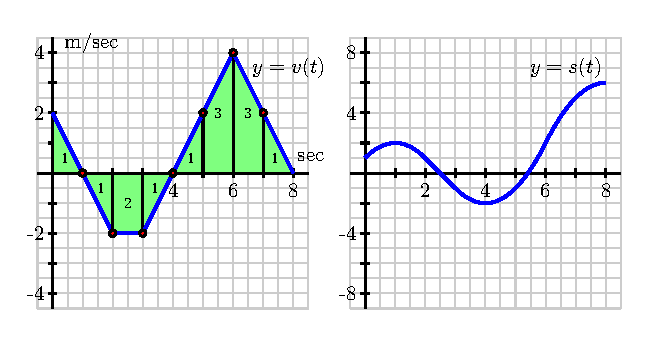
\includegraphics{figures/4_1_Act3Soln.eps}
\end{center}
\end{activitySolution}
\aftera





